\documentclass[thesis.tex]{subfiles}
\begin{document}
\chapter{AppPAL}
\label{chap:apppal}

AppPAL is an instantiation of Becker et al.'s SecPAL\cite{becker_secpal:_2010} with constraints (statements checkable using information external to the language such as the time of day or static analysis tools) and predicates that allow us to decide which apps to run or install.
The language allows us to reason about apps using statements from third parties. AppPAL allows us to enforce the policies on a device.
I can express trust relationships amongst these parties and use constraints to do additional checks, such as using security checks.
This lets us enforce more complex policies than existing tools such as Kirin which are limited to permissions checks. 
Policies can be enforced by the stores selling the apps, on the devices installing apps or by third-parties providing app vetting services.

\section{Why SecPAL?}
\label{sec:why-apppal}

For modelling and writing policies I want to start from a policy
language that supported several key features; namely:

\begin{itemize}
  \item Model decisions at separate locations.  Mobile ecosystems are
    inherently distributed, and decisions made by one device may not be
    the same as the decisions made by another device.  They may, however
    wish to share information.  By opting for a distributed language we
    can check the policies locally and make a decision based on that
    user's information rather than by deferring to an all-seeing policy
    enforcer.  This suits the problem better because individual devices
    and stores have to make decisions on their own and may not have access
    to all known information.

  \item Calling external functions that can obtain extra information
    about entities that may require special actions to fetch: for example
    an explicit ``okay'' from the user, or some metadata about an app like
    its version number.  If I don't allow the ability to fetch this
    information on-the-fly then it will have to be requested before
    checking the policy. 

    I also want to be able to use static analysis tools as part of
    our policies.  These tools can infer complex properties of apps, but
    the low-level details they check for needn't be expressable in our
    high level policies.  For example it is not necessary to encode how
    data moves over intents in AppPAL policies, but it is necessary to be
    able to say some app leaks information to another app.  A tool, such
    as FlowDroid can check for this, and there is no need to replicate the
    checking in AppPAL if I can simply call out to FlowDroid to give us a
    decision.

  \item Delegation.  I want to make a decision based on information from an
    external source.  This suggest that a \emph{can-say} mechanism is required
    that will allow us to express how trust is distributed.   Since the
    relationship between app stores and devices is one where a user delegates
    trust to the store and the device uses the external store to obtain the app
    this would hint that being able to express delegation will allow us to write
    more accurate policies.
\end{itemize}

Additionally I also wanted a language that was readable and easy to extend.
SecPAL was chosen as it met my requirements.
\todo{MORE! How did it meet my requirements? Why SecPAL over XACML/PolicyMaker/DKAL, for example}

\section{Instantiating SecPAL for mobile ecosystems}
\label{sec:instantiating}

SecPAL was designed as a generic, distributed, access control language.
To apply it to a specific domain it is necessary to instantiate the language with the necessary predicates, constraints and entities relevant to the area it will be used in.
Humphrey~\etal instantiated SecPAL with predicates for the GridFTP protocol to create a Grid access control policy language~\cite{humphrey_fine-grained_2007}.
Aziz~\etal created SecPAL4DSA by adding predicates for data-sharing agreements~\cite{aziz_secpal4dsa:_2011}.
Becker~\etal added predicates for describing \ac{PII}-handling preferences and created SecPAL4P~\cite{becker_framework_????}.
AppPAL continues in this tradition by instantiating SecPAL with predicates and constraints for mobile ecosystems, and describing app preferences.
The name emphasises this: SecPAL is a \emph{security policy authorization language}, AppPAL is an \emph{app policy authorization language}.

%\subsection{Changes from SecPAL}
AppPAL differs from SecPAL in three areas:
\begin{itemize}
  \item AppPAL predicates are given specific meaning based on their names.  
     A sugared notation is also added to aid readability, based on these conventions (\autoref{ssec:types}).
  \item AppPAL is instantiated with predicates and constraints for describing policies about apps, as well as constraints specific to Android for which AppPAL is implemented (\autoref{ssec:instantiating}).
  \item In Becker's SecPAL paper he describes an evaluation by first translating SecPAL into Datalog$^C$.
	AppPAL is evaluated by an implementation based on SecPAL's inference rules directly, however (\autoref{ssec:evaluation-alg}). \todo{WHY DID I DO THIS? (which isn't that the alg Becker describes isn't complete, and Datalog$^C$ implementations dont actually exist.}
\end{itemize}

\subsection{Typed AppPAL and Predicate Conventions}
\label{ssec:types}

SecPAL's safety condition requires all variables in an assertion's head to be
used in the body. When trying to describe policies a common pattern is to say a
variable in an assertion belongs to a certain domain. For example, Alice might
be willing to let her friends say what apps are suitable for her children. This
could be expressed in SecPAL as follows:

\begin{lstlisting}
'alice' says Friend can-say App isSuitableFor(Child)
  if Friend isFriend, App isApp, Child isChild.
\end{lstlisting}

The conditionals in this assertion add unnecessary noise to the assertion. We
know from the names of the variable what set of constants might be used
to instantiate it (Alice's \emph{friends}, \emph{apps} or \emph{children}). To
avoid this noise I added a sugared syntax to AppPAL that allows variables to
declare their \emph{type}. Using the sugared notation the above statement
becomes:

\begin{lstlisting}
'alice' says Friend:F can-say App:A isSuitableFor(Child:C).
\end{lstlisting}

\begin{figure}
  \newcommand{\nonterminal}[1]{$\langle$#1$\rangle$}
  \newcommand{\terminal}[1]{\textbf{#1}}
  \begin{tabular}{r c l}
    \footnotesize
    \nonterminal{E}         & $\coloneqq$ & \nonterminal{Variable} $\vert$ \terminal{'constant'} \\
    \nonterminal{Variable}  & $\coloneqq$ & \new{(\terminal{Type}\terminal{:})?}\terminal{VariableName}
  \end{tabular}
  \caption{Changes to SecPAL's variable syntax.  Additions are shown in \new{red}.}
  \label{fig:apppal-types}
\end{figure}

The changes to SecPAL's syntax is shown is \autoref{fig:apppal-types}.
After an assertion has been parsed the variables with types are extracted for
each variable a conditional is added that \texttt{VariableName \emph{is}Type},
and the types are removed from the variables.

This gives a cleaner policy language however it also means that the predicates
used start to have some intrinsic meaning.  A predicate starting with
\emph{is} describes some property of the predicate's subject.
SecPAL did not require predicates follow any naming conventions, however with
AppPAL we have started to give predicates meaning based on their name.

\begin{lstlisting}[language=Python, float, caption={Procedure used to expand types from AppPAL into SecPAL.}]
def expand_types(a: Assertion) -> Assertion:
  for v in a.head.vars():
    if v.type != None:
      f = Fact(v, 'is'++str(v.type))
      a.body.add(f)
  return a
\end{lstlisting}

The \emph{is} predicates give types to AppPAL variables, but there are other kinds of decisions that are useful to make when writing policies. 
By translating different policies into AppPAL four different kinds of decision were used~(\autoref{tab:predicate-prefixes}).

\newcommand{\descPred}[2]{\emph{subject} \texttt{\textbf{#1}\emph{#2}}}
\begin{table}
  \begin{tabular}{l l}
    \toprule
    Prefix                      & Meaning                                            \\
    \midrule
    \descPred{can}{Action}      & The subject is allowed to perform the action.      \\
    \descPred{has}{Action}      & The subject has performed the action.              \\
    \descPred{is}{Property}     & The property holds true for the subject.           \\
    \descPred{must}{Obligation} & The subject is required to satisfy the obligation. \\
    \bottomrule
  \end{tabular}
  \caption{Standard prefixes used for AppPAL predicates.}
  \label{tab:predicate-prefixes}
\end{table}

An \emph{is} predicate is used as described earlier, to restrict variables to a given type.
An \emph{can} predicate is used to describe permisible actions.  
For example in a \ac{BYOD} policy a company might describe what apps a device can install, and what company data a user can access.
A user might have a privacy preference describing what parts of their personal data an app can share.
App stores have procedures to go through before a developer can submit an app. \todo{CITE}
When we need to describe the conditions for an action going ahead we use the can statement.

\begin{description}
\item[\bfseries\texttt{subject \emph{is}Type}]
  A typing statement.  The \emph{subject} is an example of the \emph{type}.  An
  example might be that \lstinline!'anrgry-birds' isApp! or that
  \lstinline!'jennie' isEmployee!.
\item[\bfseries\texttt{subject \emph{has}Action}]
  A statement of action.  The \emph{subject} has carried out an \emph{action} in
  the past. For example if an app has requested a perimission then we write
  \lstinline!App:A hasRequestedPermission(Permission:P)!, if a device requires
  its owner to grant a permission we might write
  \begin{lstlisting}
'device' says User:U can-say 
  App:A hasBeenGranted(Permission:P)
  if 'device' isOwnedBy(U).
  \end{lstlisting}
\item[\bfseries\texttt{subject \emph{can}Action}]
  An authorization. The \emph{subject} is permitted to carry out the \emph{action}.
  For example \lstinline!Device:D canInstall(App:A)! to say what apps a device
  can install or \lstinline!App:A canConnectTo(URL:U)! to describe a limitation
  on app network abilities.
\item[\bfseries\texttt{subject \emph{must}Action}]
  An obligation.  The \emph{subject} should carry out the \emph{action} as soon
  as possible.
  An example might be requiring the device inform a company's IT department if
  there have been three unsuccessful password attempts:
  \begin{lstlisting}
'company' says Device:D mustInform('it', 'login-failure')
  if D hasUnsuccesfulLogins(N)
  where N >= 3.
  \end{lstlisting}
\end{description}

This differs slightly from the approach taken with the SecPAL4P and SecPAL4DSA~\cite{becker_framework_????,aziz_secpal4dsa:_2011} instantiations.
Both these languages add additional special phrases to SecPAL's grammar.
For example SecPAL4P adds a \emph{may} and \emph{will} phrase to describe whether a behavior could or will be carried out.
If Alice, a policy author, wished to use SecPAL4P to say that someone can forget her email address she could write:\footnote{%
  Example taken from~\cite{becker_framework_????}.  SecPAL4P also has relaxed safety rules, that permit the variables $x$ and $t$ to be in the head of the rule, but not the body.}
\begin{lstlisting}
Alice says x may delete Email within t
\end{lstlisting}
An analogous AppPAL rule would be:
\begin{lstlisting}
'alice' says User:X canDeleteWithin('email', Time:t)
  where currentTime() < t.
\end{lstlisting}
The AppPAL is arguably slightly less readable, but more explicit than the SecPAL4DSA.
Because AppPAL has less special cases the syntax is simpler also.

\subsection{Instantiating SecPAL for mobile ecosystems}
\label{ssec:instantiating}

\subsection{Instantiating SecPAL for BYOD}

\subsection{Evaluation}
\label{ssec:evaluation-alg}

To implement AppPAL I chose to implement the inference rules directly rather than rely on a translation to Datalog$^C$.
This avoids the need to rely on a Datalog$^C$ implementation, which are not readily available.
It also means the implementation can be optimized for AppPAL's specific evaluation rules.

Given an \ac{AC}, a policy file containing AppPAL facts and rules, we extract three sets of constant.
If a constant is used before a \emph{says} statement, or it is used as the subject of a \emph{can-say} fact then the constant is marked as \emph{voiced}.  
If the constant is used immediately after the \emph{says} or as the subject of a fact then it is marked as a \emph{subject}.
We also make use of a results table to store partial results and previously established proofs.
The table is indexed by queries and a delegation depth, partial results (i.e. that a query is being evaluated).
This allows previous results to reused without recomputation or constraint re-evaluation, and when evaluation has entered a loop.
All ground facts in the assertion context are automatically added to the results table.
This results table is shared between evaluations of an \ac{AC}.
Finally we take a list of all the predicates used in the \ac{AC}.
If we have a statement that allows us to make a statement about an assertion then we mark it as \emph{derviable}.

\begin{table}
  \centering
  \newcommand{\myset}[1]{\ensuremath{\text{\sffamily #1}}}
  \begin{tabular}{r l c}
    \toprule
    $c \in \myset{Voiced} \impliedby$     & $\exists \left(c \text{~says~} \cdots\right) \in \text{AC}$                        & $\bigvee$ \\
                                          & $\exists \left(\star \text{~says~} c \text{~can-say~} \cdots\right) \in \text{AC}$ &           \\
    $c \in \myset{Subjects} \impliedby$   & $\exists \left(\star \text{~says~} c\cdots\right) \in \text{AC}$                   & $\bigvee$ \\
                                          & $\exists \left(\cdots \text{~if~} \cdots,c~\star,\cdots\right) \in \text{AC},$     &           \\
                                          & $c \in \myset{Constants}$                                                          &           \\
    $p \in \myset{Derivable} \impliedby$  & $\exists \left( \cdots \star~p\left(\cdots\right) \cdots\right) \in \text{AC}$     &           \\
    \bottomrule                          \\
  \end{tabular}
  \caption{Sets used in AppPAL evaluation.}
\end{table}


\todo{this is taken from the AppPAL for Android paper, but I don't like it.  Redo more abstractly.}
\begin{lstlisting}[language=Python, float, caption={Pseudocode for evaluating AppPAL.}]
def evaluate(ac, rt, q, d):
  return rt[q, d] if rt.contains((q, d))
  p = cond(ac, rt, q, d)
  result = None
  if p.isValid():
    rt[q, d] = p 
    result = Proven
  else:
    p = canSay_CanActAs(ac, rt, q, d)
    if p.isValid():
      rt[q, d] = p 
      result = Proven
    else:
      rt[q, d] = Failure
      result = Failure
  return (result, rt)

def cond(ac, rt, q, d):
  ac.add(q.fetch()) if q.isFetchable()
  for a in ac.assertion():
    u = q.unify(a.consequent)
    if u.isValid:
      a = u.apply(a)
      if (a.variables() == None):
        return checkConditions(ac, rt, a, d)
  return Failure

def canSay_canActAs(ac, rt, q, d):
  for c in ac.constants():
    if ac.subject(c):
      p = canActAs(ac, rt, q, d)
      return Proven if p.isValid()
    elif ac.speaker(c):
      p = canSay(ac, rt, q, d)
      return Proven if p.isValid
  return Failure

def checkConditions(ac, rt, a, d):
  for s in getVarSubs(a, ac.constants()):
    sa = s.apply(a)
    if sa.body().all(lambda a: evaluate(ac, rt, a, d).isValid()):
      p = evaluateConstraint(sa.constraint())
      return Proven is p.isValid()
  return Failure
\end{lstlisting}

\section{Examples of AppPAL}

Consider the following example: a user, Alice, may have rules she has to follow
when using apps for work and her own policies when using apps at home in her
private life. Using AppPAL I can write policies for work and home, and decide
which policy to enforce using a user's location, or the time of day:

\begin{lstlisting}
'alice' says App isRunnable
  if 'home-policy' isMetBy(App)
  where at('work') = false.

'alice' says App isRunnable
  if 'work-policy' isMetBy(App)
  where beforeHourOfDay('17') = true.
\end{lstlisting}

I can delegate policy specification to third parties or roles, and assign principals to roles:

\begin{lstlisting}
'alice' says 'it-department' can-say 'work-policy' isMetBy(App).
'alice' says 'alice' can-act-as 'it-department'.
\end{lstlisting}

I can write policies specifying which permissions an app must or must not have
by its app store categorization. For example, it would be okay allowing a
photography app access to the camera, but not to allow access to location data
if the user doesn't want their photos geotagged.

\begin{lstlisting}
'alice' says App isRunnable
  if 'permissions-policy' isMetBy(App).
'alice' says 'permissions-policy' isMetBy(App)
  if App isAnApp
  where
    category(App, 'Photography'),
    hasPermission(App, 'LOCATION') = false,
    hasPermission(App, 'CAMERA') = true.
\end{lstlisting}

\section{Implementation}

AppPAL is implemented as a library for Android and Java.
The parser is implemented using ANTLR4.

\subsection{Benchmarks}
\label{ssec:benchmarks}

If AppPAL were to run on a mobile phone, apps should be checked as they are installed.
Since policy checks may involve inspecting many rules and constraints one may ask whether the checking will be acceptably fast.
Downloading and installing an app takes about 30 seconds on a typical Android phone over wifi.
If checking a policy delays this even further a user may become annoyed and disable AppPAL.

To give a measure the performance of AppPAL a synthetic benchmark was developed.
The policy checking procedure is at its slowest when having to delegate repeatedly;
the depth of the delegation tree is the biggest factor for slowing the search.
Synthetic benchmarks were created to check that the checking procedure performed acceptably.
Each benchmark consisted of a chain of delegations.
The \emph{1 to 1} benchmark consists of a repeated delegation between all the principals.
In the \emph{1 to 2} benchmark each principal delegated to 2 others and in the \emph{1 to 3} benchmark each principal delegated to 3 others.
These benchmarks are reasonable as they model the slowest kinds of policies to
evaluate---though worse ones could be designed by delegating even more or triggering an expensive constraint check.o

For each benchmark we controlled the number of principals in the policy file:
as the number of principals increased so did the size of the policy.
The results are shown in \autoref{tab:benchmarks}.
Most typical policies (such as those discussed in \autoref{chap:apps-and-stores} and \autoref{chap:byod}), use only few delegations per decision.
I believe the policy checking performance of AppPAL is acceptable as unless a policy consists of hundreds of delegating principals the overhead of checking an AppPAL policy is negligable, even on a power constrained device such as a mobile phone.

\begin{table}
  \centering\sffamily
    \begin{tabular}{c c r@{.}l}
      \toprule
      Delegations & Principals & \multicolumn{2}{c}{Time (s)} \\
      \midrule
      1 to 1 & 10   &  0&01 \\
      1 to 1 & 100  &  1&00 \\
      1 to 1 & 500  & 20&90 \\
      1 to 1 & 1000 & 88&73 \\
      \midrule
      1 to 2 & 10   &  0&01 \\
      1 to 2 & 100  &  0&43 \\
      1 to 2 & 500  &  7&36 \\
      1 to 2 & 1000 & 27&47 \\
      \midrule
      1 to 3 & 10   &  0&01 \\
      1 to 3 & 100  &  0&24 \\
      1 to 3 & 500  &  3&99 \\
      1 to 3 & 1000 & 15&28 \\
      \bottomrule
    \end{tabular}
    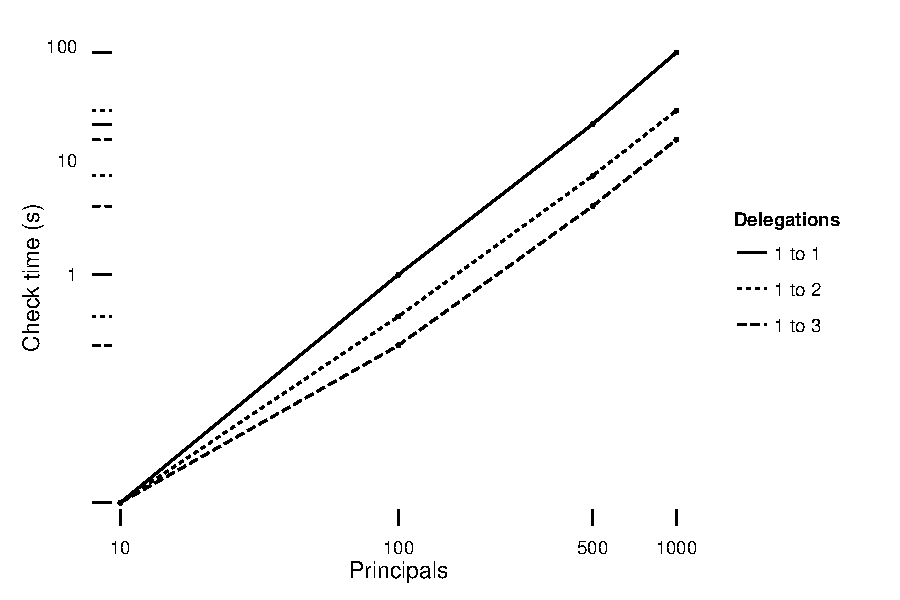
\includegraphics[width=0.70\linewidth]{figures/benchmarks.pdf}
  \caption{Benchmarking results on a Nexus 4 Android phone.}
  \label{tab:benchmarks}
\end{table}

\end{document}

%%% Local Variables:
%%% mode: latex
%%% TeX-master: "../thesis"
%%% End:
